\chapter{Establishing a Baseline}
\label{ch:baseline}

This chapter covers the first stage of the work: obtaining a decentralized
MAPPO agent that trains stably on the IEEE 14-bus task, and then testing
whether replacing its flat MLP actor with a graph encoder is worth the added
complexity. Everything here maximizes survival; the representation is fixed and
deliberately simple.
\\
\\
Its conclusion sets up the two chapters that follow. If a graph encoder helps,
the next question is which graph, which is what Chapter~\ref{ch:methods} defines
and Chapter~\ref{ch:experiments} screens.

\section{How to Read This Chapter}
\label{sec:results-structure}

This chapter is organized as a sequence of experiment blocks, and the later
experimental chapters reuse the same pattern. Each block follows the same
structure:

\begin{enumerate}
  \item \textbf{Question.} What uncertainty or design choice does this test
  address?
  \item \textbf{Baseline and change.} Which run is the control, and what is
  changed in the comparison runs?
  \item \textbf{Protocol.} Which data split, checkpoint, seeds, and metric are
  used?
  \item \textbf{Implementation detail.} Which algorithmic, architectural, or
  mathematical change is being tested, when this is relevant?
  \item \textbf{Evidence.} Which table and figure summarize the result?
  \item \textbf{Interpretation.} What can be concluded, and what still needs to
  be verified?
\end{enumerate}

\section{Evaluation Protocol}
\label{sec:results-evaluation-protocol}

The experiments use a train/test chronic split. The training set contains
80\% of the chronics and is used to update the policy. The test set contains
the remaining 20\% and is used to estimate generalization during training and
for final evaluation.
\\
\\
During training, evaluation rollouts are periodically run on both the train and
test splits using 10 episodes each time. In the current rerun notebook, the main
reported metric is \textbf{test episodic survival}, expressed as a percentage. 
Higher survival means that the agent keeps the grid alive for a larger fraction 
of the evaluation episodes. The final plots show seed-aggregated mean curves, 
faint individual seed curves, and the variability band.
\\
\\
The final evaluation currently uses the saved checkpoint with the best test survival. This selection rule should be reported explicitly because
the test split participates in checkpoint selection; the values in this chapter
are therefore best interpreted as controlled rerun comparisons, not as a final
untouched test-set estimate.

\section{Experiment Index}
\label{sec:results-experiment-index}

Table~\ref{tab:experiment-index} maps the experiment blocks of this chapter.
The sparse-control experiments follow a different objective and are reported
separately in Chapter~\ref{ch:sparse-control}.

\begin{table}[H]
  \centering
  \small
  \caption{Current result blocks and their role in the thesis.}
  \label{tab:experiment-index}
  \setlength{\tabcolsep}{4pt}
  \begin{tabular}{L{0.17\textwidth}L{0.34\textwidth}L{0.32\textwidth}L{0.10\textwidth}}
    \toprule
    Block & Main question & Primary evidence & Status \\
    \midrule
    A0 core reruns & Which baseline training changes stabilize MAPPO? &
    Table~\ref{tab:a0-core-summary}, Figures~\ref{fig:rerun-a0-pairwise}
    and~\ref{fig:rerun-a0-all} & Drafted \\
    Initial do-nothing bias & Does an initial action-0 prior help exploration? &
    Table~\ref{tab:a0-bias-summary}, Figure~\ref{fig:rerun-a0-bias} & Drafted \\
    GINE reruns & Do graph encoders improve survival over the A0 baseline? &
    Tables~\ref{tab:gine-run-configurations} and~\ref{tab:gine-rerun-summary},
    Figure~\ref{fig:rerun-gine-best00} & Drafted \\
    Heavy GINE & Does a larger GINE architecture help or overcomplicate
    optimization? & Table~\ref{tab:heavy-gine-configurations},
    Figure~\ref{fig:gine-best-search2} & Drafted \\
    \bottomrule
  \end{tabular}
\end{table}

\section{IEEE 14-Bus Experiments}
\label{sec:bus14-results}

The first result group focuses on the IEEE 14-bus topology-control task. The
initial PPO/MAPPO baseline from the MARL2Grid framework was not satisfactory:
the agents did not learn a robust policy and the survival rate remained low.
The following experiments therefore test training and architecture changes that
could make the baseline more stable.

\subsection{A0 Core Reruns}
\label{subsec:a0-core-reruns}

\paragraph{Question.}
Which changes are needed to obtain a stable MLP MAPPO baseline on the 14-bus
task?

\paragraph{Baseline and changes.}
The A0 family starts from the flat MLP MAPPO baseline and tests three main
stabilization choices:

\begin{itemize}
  \item increasing actor and critic capacity from two hidden layers to three
  hidden layers;
  \item using reward normalization;
  \item changing the critic update so that the critic is updated once for the
  whole batch instead of once per agent.
\end{itemize}

\paragraph{Implementation detail.}
There is no new mathematical objective in this ablation. The implementation
changes are practical training choices: network depth, reward normalization,
critic-update scheduling, and the initialization of the action-0 probability.
Table~\ref{tab:a0-run-configurations} records these settings so that the
survival plots can be interpreted without repeatedly restating the run names.

\paragraph{Evidence.}
Table~\ref{tab:a0-core-summary} reports final and peak survival for the core A0
ablations. Figure~\ref{fig:rerun-a0-pairwise} shows each comparison against the
\texttt{rerun\_a0\_opt} baseline, and Figure~\ref{fig:rerun-a0-all} overlays all
core A0 curves.

\paragraph{Interpretation.}
The optimized A0 baseline, the non-optimized critic-update variant, and the
smaller MLP variant all finish around \(93\%\) survival. This suggests that the
main A0 recipe is robust once the rerun protocol is fixed. Disabling reward
normalization still reaches high peak survival, but it learns more slowly and
finishes lower. The old no-validation, non-optimized baseline is clearly not
competitive and should not be used as the main reference for later ablations.

\begin{table}[H]
  \centering
  \scriptsize
  \caption{A0-family run configurations. The reference run is
  \texttt{rerun\_a0\_opt}.}
  \label{tab:a0-run-configurations}
  \setlength{\tabcolsep}{3pt}
  \begin{tabular}{L{0.21\textwidth}L{0.13\textwidth}L{0.10\textwidth}L{0.12\textwidth}L{0.12\textwidth}L{0.22\textwidth}}
    \toprule
    Run family & Actor/critic hidden layers & Reward norm. & Initial action-0 prob. &
    Optimized critic update & Difference from \texttt{rerun\_a0\_opt} \\
    \midrule
    \texttt{rerun\_a0\_opt} & \(3\times256\) / \(3\times256\) &
    true & 0.0 & true & Reference baseline \\
    \texttt{rerun\_a0\_nonopt} & \(3\times256\) / \(3\times256\) &
    true & 0.0 & false & Disables optimized critic updates \\
    \texttt{rerun\_a01} & \(2\times256\) / \(2\times256\) &
    true & 0.0 & true & Uses a smaller MLP actor and critic \\
    \texttt{rerun\_a02} & \(3\times256\) / \(3\times256\) &
    false & 0.0 & true & Disables reward normalization \\
    \texttt{old\_a0\_nonopt\_noval20} & \(3\times256\) / \(3\times256\) &
    true & 0.3 & false & Uses action-0 bias 0.3 and non-optimized critic updates \\
    \texttt{rerun\_bias\_05} & \(3\times256\) / \(3\times256\) &
    true & 0.5 & true & Uses action-0 bias 0.5 \\
    \texttt{rerun\_bias\_07} & \(3\times256\) / \(3\times256\) &
    true & 0.7 & true & Uses action-0 bias 0.7 \\
    \bottomrule
  \end{tabular}
\end{table}

\begin{figure}[H]
  \centering
  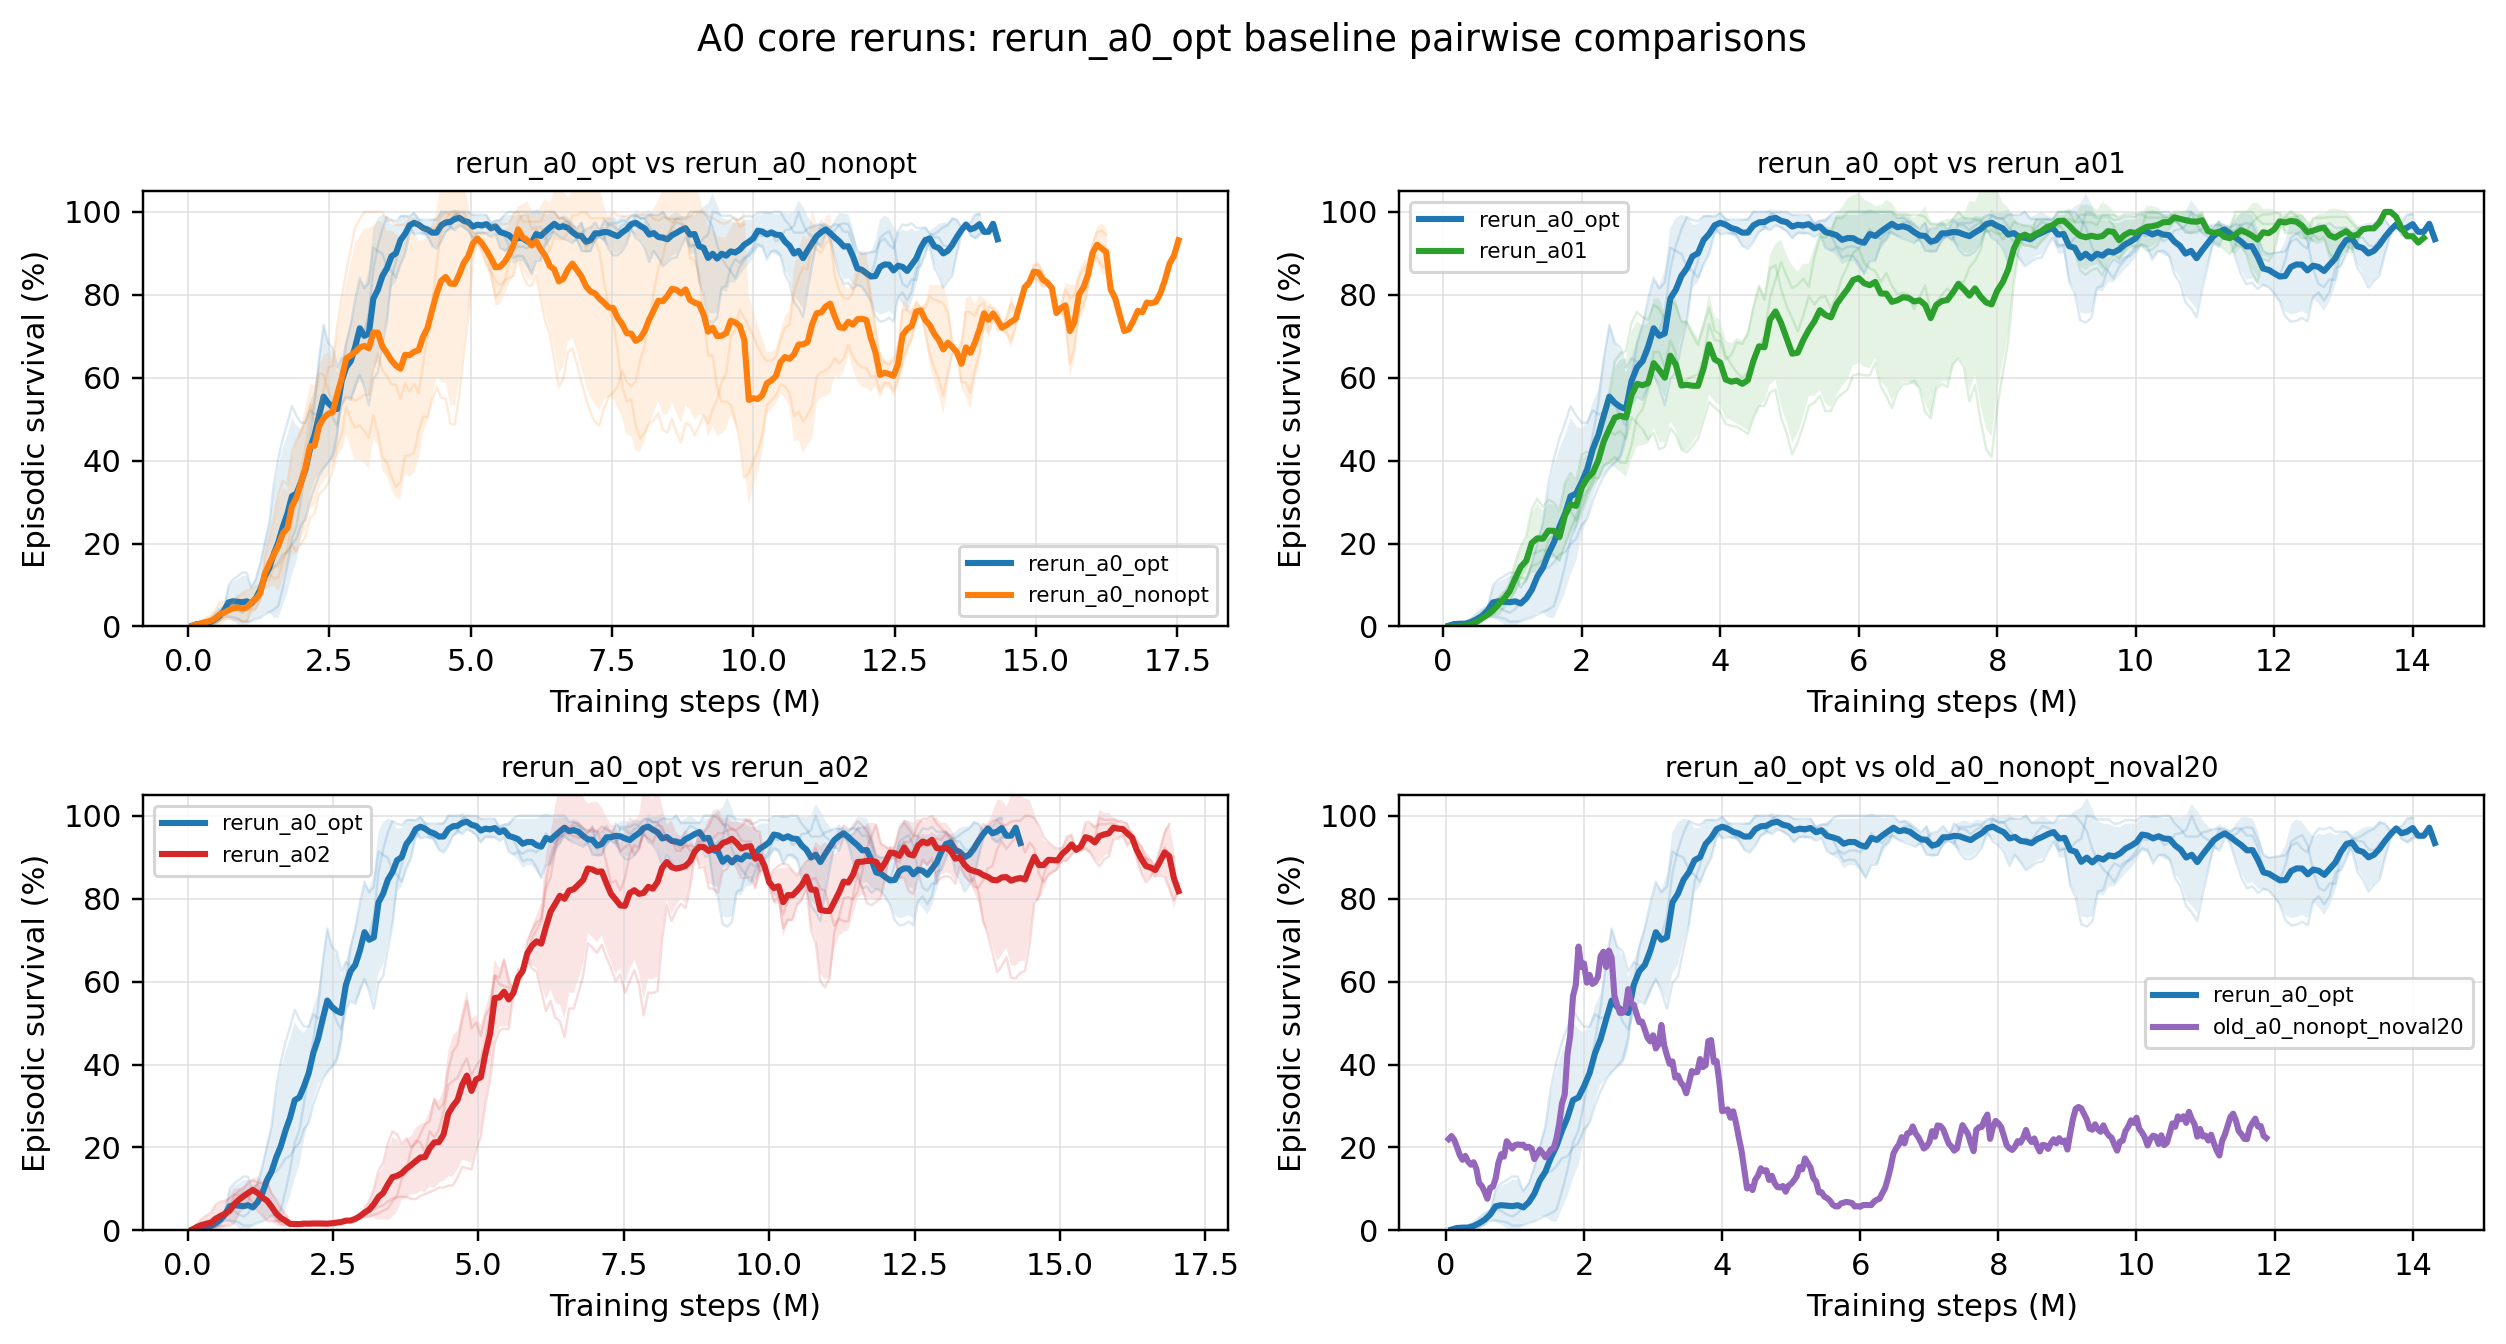
\includegraphics[width=\textwidth]{figures/rerun_a0_core_pairwise_comparisons.png}
  \caption{Pairwise A0 rerun comparisons against the \texttt{rerun\_a0\_opt}
  baseline.}
  \label{fig:rerun-a0-pairwise}
\end{figure}

\begin{figure}[H]
  \centering
  
\includegraphics[width=\textwidth]{figures/rerun_a0_core_all_curves.png}
  \caption{All A0 core rerun survival curves shown on one axis.}
  \label{fig:rerun-a0-all}
\end{figure}

\begin{table}[H]
  \centering
  \small
  \caption{A0 core rerun survival summary.}
  \label{tab:a0-core-summary}
  \resizebox{\textwidth}{!}{%
  \begin{tabular}{llrr}
    \toprule
    Run & Intended change & Final survival (\%) & Peak survival (\%) \\
    \midrule
    \texttt{rerun\_a0\_opt} & A0 optimized baseline & 93.4 & 98.6 \\
    \texttt{rerun\_a0\_nonopt} & Disable optimized critic update & 93.1 & 95.8 \\
    \texttt{rerun\_a01} & Smaller MLP actor/critic & 93.7 & 100.0 \\
    \texttt{rerun\_a02} & Disable reward normalization & 81.8 & 97.1 \\
    \texttt{old\_a0\_nonopt\_noval20} & Older non-optimized protocol & 22.3 & 68.4 \\
    \bottomrule
  \end{tabular}
  }
\end{table}

\subsection{Initial Do-Nothing Bias}
\label{subsec:a0-bias-reruns}

\paragraph{Question.}
Does biasing the initial policy toward action 0, the do-nothing action, help or
hurt learning?

\paragraph{Baseline and changes.}
The A0 baseline uses no initial do-nothing bias in this rerun set. The bias
controls keep the same general protocol but change the initial probability mass
assigned to action 0.


\paragraph{Implementation detail.}
The bias is applied only at initialization: it changes the starting action
distribution before learning, without changing the reward, architecture, or PPO
objective. This makes the ablation a test of exploration bias rather than a test
of representational capacity.

\paragraph{Evidence.}
Table~\ref{tab:a0-bias-summary} and Figure~\ref{fig:rerun-a0-bias} compare the
zero-bias A0 baseline with \texttt{rerun\_bias\_05} and
\texttt{rerun\_bias\_07}.

\paragraph{Interpretation.}
The effect of the action-0 bias is large and non-monotonic. The 0.5-bias curve
remains unstable and substantially below the zero-bias baseline, whereas the
0.7-bias curve eventually reaches the highest final survival in this comparison.
The current conclusion is therefore not that larger bias is always better.
Instead, the initialization prior appears to strongly shape exploration and
should be treated as a first-order ablation variable.

\begin{table}[H]
  \centering
  \small
  \caption{Initial do-nothing bias survival summary.}
  \label{tab:a0-bias-summary}
  \begin{tabular}{lrr}
    \toprule
    Run & Final survival (\%) & Peak survival (\%) \\
    \midrule
    \texttt{rerun\_a0\_opt} & 93.4 & 98.6 \\
    \texttt{rerun\_bias\_05} & 50.8 & 70.2 \\
    \texttt{rerun\_bias\_07} & 99.3 & 100.0 \\
    \bottomrule
  \end{tabular}
\end{table}

\begin{figure}[H]
  \centering
  
\includegraphics[width=\textwidth]{figures/rerun_a0_bias_comparison.png}
  \caption{A0 baseline compared with initial do-nothing bias controls
  \texttt{rerun\_bias\_05} and \texttt{rerun\_bias\_07}.}
  \label{fig:rerun-a0-bias}
\end{figure}


\subsection{GINE Encoder Reruns}
\label{subsec:gine-reruns}

\paragraph{Question.}
Can graph encoders improve topology-control performance, and which GINE design
choices matter most?

\paragraph{Baseline and changes.}
The comparison starts from the historical \texttt{best\_00} GINE baseline. The
reruns then test lighter GINE encoders, MLP versus GNN critics, optimized critic
updates, flat-feature concatenation, A0-style entropy, and different
do-nothing-bias settings.

\paragraph{Protocol.}
All GINE runs use \texttt{gnn\_type = gine}, reward normalization,
\(15{,}000{,}000\) total timesteps, evaluation every \(80{,}000\) timesteps,
\(2{,}000\) rollout steps, deterministic evaluation, and the same 80/20 chronic
split used by the A0 experiments. The reference run is \texttt{best\_00}.

\paragraph{Implementation detail.}
The complete GINE/GAT graph-actor pipeline, including edge-conditioned message
passing, pooling, and the action head, is described in
Appendix~\ref{app:gine-architecture}. This block separates representational
changes from optimization changes. The GINE encoder changes how grid
observations are embedded, while the critic type, flat-feature concatenation,
entropy setting, and critic-update schedule affect how the PPO objective is
optimized.

\paragraph{Evidence.}
Table~\ref{tab:gine-run-configurations} records the run configurations,
Table~\ref{tab:gine-rerun-summary} gives the selected survival values, and
Figure~\ref{fig:rerun-gine-best00} shows the pairwise survival curves against
\texttt{best\_00}.

\paragraph{Interpretation.}
The strongest GINE result is \texttt{best\_14}, which reaches about
\(95.7\%\) final survival. This suggests that the graph encoder can be
competitive when it is paired with a simpler MLP critic and stable A0-style
training choices. The heavier historical GINE baseline has high peak survival
but much weaker final survival, which points to optimization stability rather
than representational capacity as the main issue.

\begin{landscape}
\begin{table}[p]
  \centering
  \scriptsize
  \caption{GINE rerun configuration summary. The reference run is
  \texttt{best\_00}.}
  \label{tab:gine-run-configurations}
  \setlength{\tabcolsep}{2.4pt}
  \renewcommand{\arraystretch}{1.12}
  \begin{tabular}{L{0.095\linewidth}L{0.075\linewidth}L{0.065\linewidth}L{0.095\linewidth}L{0.050\linewidth}L{0.060\linewidth}L{0.050\linewidth}L{0.065\linewidth}L{0.070\linewidth}L{0.275\linewidth}}
    \toprule
    Run & Actor/critic encoder & GNN hidden/layers & Actor/critic heads &
    Concat flat & Edge pre-enc. & Entropy & Init action-0 & Opt. critic &
    Difference from \texttt{best\_00} \\
    \midrule
    \texttt{best\_00} & \texttt{gnn} / \texttt{gnn} & 128 / 2 &
    \(3\times256\) / \(3\times256\) & true & true & 0.02 & 0.7 & false &
    Baseline: heavy concat-flat GINE actor, GNN critic, and legacy critic updates \\
    \texttt{best\_10} & \texttt{gnn} / \texttt{mlp} & 64 / 1 &
    \(2\times128\) / \(2\times128\) & true & false & 0.02 & 0.7 & true &
    Light GINE actor, MLP critic, smaller heads, no edge pre-encoder, optimized critic updates \\
    \texttt{best\_11} & \texttt{gnn} / \texttt{gnn} & 128 / 2 &
    \(3\times256\) / \(3\times256\) & true & true & 0.02 & 0.0 & false &
    Bias ablation: same as baseline, but the initial do-nothing prior is 0.0 \\
    \texttt{best\_12} & \texttt{gnn} / \texttt{gnn} & 128 / 2 &
    \(3\times256\) / \(3\times256\) & true & true & 0.02 & 0.0 & true &
    Bias 0.0 plus optimized critic updates; otherwise heavy concat-flat GINE with GNN critic \\
    \texttt{best\_13} & \texttt{gnn} / \texttt{gnn} & 128 / 2 &
    \(3\times256\) / \(3\times256\) & true & true & 0.01 & 0.0 & true &
    A0-style heavy GINE: bias 0.0, lower entropy 0.01, optimized critic updates \\
    \texttt{best\_14} & \texttt{gnn} / \texttt{mlp} & 64 / 1 &
    \(2\times128\) / \(2\times128\) & false & false & 0.01 & 0.0 & true &
    Light A0-style GINE: MLP critic, no concat-flat, lower entropy 0.01, bias 0.0, optimized critic updates \\
    \bottomrule
  \end{tabular}
\end{table}
\end{landscape}

\begin{table}[H]
  \centering
  \small
  \caption{GINE rerun survival summary.}
  \label{tab:gine-rerun-summary}
  \resizebox{\textwidth}{!}{%
  \begin{tabular}{llrr}
    \toprule
    Run & Intended change & Final survival (\%) & Peak survival (\%) \\
    \midrule
    \texttt{best\_00} & Historical GINE baseline & 59.2 & 93.9 \\
    \texttt{best\_10} & Light GINE with MLP critic & 78.9 & 90.4 \\
    \texttt{best\_12} & Optimized critic and bias 0.0 & 82.5 & 85.7 \\
    \texttt{best\_14} & Light A0-style GINE with MLP critic & 95.7 & 97.4 \\
    \bottomrule
  \end{tabular}
  }
\end{table}

\begin{figure}[H]
  \centering
  
\includegraphics[width=\textwidth]{figures/rerun_gine_best00_vs_best10_14.png}
  \caption{Seed-aggregated test episodic survival for GINE
  \texttt{best\_00} against \texttt{best\_10}--\texttt{best\_14}.}
  \label{fig:rerun-gine-best00}
\end{figure}

\subsection{Heavy GINE}
\label{subsec:heavy-gine}

\paragraph{Question.}
Does the heavier concat-flat GINE baseline fail because it lacks capacity, or
because specific architectural and optimization choices make it unstable?

\paragraph{Baseline and changes.}
The reference run is \texttt{best\_00}, the historical shared-actor,
concat-flat GINE with a GNN critic and legacy critic updates. The best-search 2
family compares this baseline against controlled alternatives that change the
flat-feature concatenation, critic type, actor sharing, GNN size, entropy
schedule, node identifiers, message-passing operator, and initialization bias.

\paragraph{Protocol.}
The configurations are read from
\texttt{configs/gine\_s0\_s1\_s2}. Each family is run with seeds
\texttt{s0}, \texttt{s1}, and \texttt{s2}. Unless changed by the family, the
runs use reward normalization, deterministic evaluation, 5 evaluation episodes,
\(15{,}000{,}000\) total timesteps, evaluation every \(80{,}000\) timesteps, and
the same 80/20 chronic split.

\paragraph{Implementation detail.}
Table~\ref{tab:heavy-gine-configurations} gives the parameter comparison used
for this ablation. The table is based on the \texttt{s0} TOML file for each
family; the corresponding \texttt{s1} and \texttt{s2} files keep the same
configuration except for the training seed and run name.

\paragraph{Evidence.}
Figure~\ref{fig:gine-best-search2} compares the \texttt{best\_00} baseline
against each heavy-GINE alternative. Each panel shows the seed-averaged
test-survival curve for \texttt{best\_00} and one comparison family, with faint
seed curves and variability bands.

\paragraph{Interpretation.}
The broad search suggests that the heavy baseline is not limited by capacity
alone. Several simpler or more constrained variants improve final survival over
\texttt{best\_00}, especially removing node-ID embeddings, removing flat
concatenation, using an MLP critic, and combining a light GINE actor with an MLP
critic. In contrast, simply switching message passing to GAT or weighted GCN,
or removing the initial do-nothing bias while keeping the heavy GINE/GNN-critic
structure, does not clearly solve the stability problem.


\begin{landscape}
\begin{table}[p]
  \centering
  \tiny
  \caption{Heavy-GINE best-search 2 parameter comparison from
  \texttt{configs/gine\_s0\_s1\_s2}.}
  \label{tab:heavy-gine-configurations}
  \setlength{\tabcolsep}{2pt}
  \renewcommand{\arraystretch}{1.12}
  \begin{tabular}{L{0.065\linewidth}L{0.215\linewidth}L{0.045\linewidth}L{0.060\linewidth}L{0.050\linewidth}L{0.075\linewidth}L{0.045\linewidth}L{0.045\linewidth}L{0.045\linewidth}L{0.045\linewidth}L{0.060\linewidth}L{0.045\linewidth}L{0.055\linewidth}}
    \toprule
    Run & Main change from \texttt{best\_00} & GNN & GNN size & Critic &
    Actor/critic heads & Concat & Shared & Edge pre. & Node ID & Entropy &
    Init action-0 & Opt. critic \\
    \midrule
    \texttt{best\_000} & Removes flat-observation concatenation &
    \texttt{gine} & \(2\times128\) & \texttt{gnn} & \(3\times256\) / \(3\times256\) &
    no & yes & yes & yes & 0.02--0.02 & 0.7 & no \\
    \texttt{best\_00} & Reference: heavy concat-flat GINE with GNN critic &
    \texttt{gine} & \(2\times128\) & \texttt{gnn} & \(3\times256\) / \(3\times256\) &
    yes & yes & yes & yes & 0.02--0.02 & 0.7 & no \\
    \texttt{best\_01} & Enables optimized critic updates &
    \texttt{gine} & \(2\times128\) & \texttt{gnn} & \(3\times256\) / \(3\times256\) &
    yes & yes & yes & yes & 0.02--0.02 & 0.7 & yes \\
    \texttt{best\_02} & Replaces the GNN critic with an MLP critic &
    \texttt{gine} & \(2\times128\) & \texttt{mlp} & \(3\times256\) / \(3\times256\) &
    yes & yes & yes & yes & 0.02--0.02 & 0.7 & no \\
    \texttt{best\_03} & Uses non-shared actor GNN weights &
    \texttt{gine} & \(2\times128\) & \texttt{gnn} & \(3\times256\) / \(3\times256\) &
    yes & no & yes & yes & 0.02--0.02 & 0.7 & no \\
    \texttt{best\_04} & Uses a lighter GINE encoder &
    \texttt{gine} & \(1\times64\) & \texttt{gnn} & \(3\times256\) / \(3\times256\) &
    yes & yes & yes & yes & 0.02--0.02 & 0.7 & no \\
    \texttt{best\_05} & Decays entropy from 0.02 to 0.0 &
    \texttt{gine} & \(2\times128\) & \texttt{gnn} & \(3\times256\) / \(3\times256\) &
    yes & yes & yes & yes & 0.02--0.00 & 0.7 & no \\
    \texttt{best\_06} & Removes learned node-ID embeddings &
    \texttt{gine} & \(2\times128\) & \texttt{gnn} & \(3\times256\) / \(3\times256\) &
    yes & yes & yes & no & 0.02--0.02 & 0.7 & no \\
    \texttt{best\_07} & Replaces GINE with GAT message passing &
    \texttt{gat} & \(2\times128\) & \texttt{gnn} & \(3\times256\) / \(3\times256\) &
    yes & yes & yes & yes & 0.02--0.02 & 0.7 & no \\
    \texttt{best\_08} & Replaces GINE with weighted GCN message passing &
    \texttt{gcn} & \(2\times128\) & \texttt{gnn} & \(3\times256\) / \(3\times256\) &
    yes & yes & yes & yes & 0.02--0.02 & 0.7 & no \\
    \texttt{best\_09} & Light no-concat GINE with MLP critic and optimized critic updates &
    \texttt{gine} & \(1\times64\) & \texttt{mlp} & \(2\times128\) / \(2\times128\) &
    no & yes & no & yes & 0.02--0.02 & 0.7 & yes \\
    \texttt{best\_10} & Light concat-flat GINE with MLP critic and optimized critic updates &
    \texttt{gine} & \(1\times64\) & \texttt{mlp} & \(2\times128\) / \(2\times128\) &
    yes & yes & no & yes & 0.02--0.02 & 0.7 & yes \\
    \texttt{best\_11} & Removes the initial do-nothing bias &
    \texttt{gine} & \(2\times128\) & \texttt{gnn} & \(3\times256\) / \(3\times256\) &
    yes & yes & yes & yes & 0.02--0.02 & 0.0 & no \\
    \bottomrule
  \end{tabular}
\end{table}
\end{landscape}

\begin{landscape}
\begin{figure}[p]
  \centering
  
\includegraphics[width=\linewidth,height=0.86\textheight,keepaspectratio]{figures/gine_best_search2_baseline_comparisons.png}
  \caption{Heavy-GINE best-search 2 survival comparisons. Each subplot compares
  the \texttt{best\_00} heavy concat-flat GINE baseline against one controlled
  alternative from \texttt{configs/gine\_s0\_s1\_s2}.}
  \label{fig:gine-best-search2}
\end{figure}
\end{landscape}

